\documentclass[12pt]{report}
\usepackage[a4paper, total={16cm, 24cm}]{geometry}
\usepackage[greek]{babel}	
\usepackage[Glenn]{fncychap}
\usepackage[version=4]{mhchem}
\usepackage[backend=biber, sorting=none]{biblatex}
\usepackage{listings}
\usepackage{multicol}
\usepackage{xcolor}
\usepackage{caption}
\usepackage{subcaption}
\usepackage{graphicx}
\usepackage{wrapfig}
\usepackage{gfsdidot}
\usepackage{sidecap}
\usepackage{enumitem}
\usepackage{pgfornament}

\addbibresource{thesis.bib}
\graphicspath{{img/}}

\definecolor{codegray}{rgb}{0.5,0.5,0.5}
\definecolor{backcolour}{rgb}{0.95, 0.95, 0.92}

\lstdefinestyle{style}{
    backgroundcolor=\color{backcolour},   
    basicstyle=\ttfamily\footnotesize,
    breakatwhitespace=false,         
    breaklines=true,                 
    keepspaces=true,                 
    showspaces=false,                
    showstringspaces=false,
    showtabs=false,                  
    tabsize=2
}
\lstset{style=style}

\author{Βεϊσάκης Μανούσος}
\title{Μοντελοποίηση συστημάτων αποθήκευσης, \\με σκοπό την αυξημένη διείσδυση των ΑΠΕ \\στο δίκτυο ηλεκτρικής ενέργειας}
\date{\today}

\begin{document}
\maketitle
\tableofcontents
\chapter*{Ευχαριστίες}
\chapter*{{\latintext{Abstract}}}
Η μεταστροφή σε φιλικότερες για το περιβάλλον πηγές ενέργειας είναι αναπόφευκτη, καθώς η ανάγκη για ένα οικολογικότερο μέλλον, αλλά και η επιβάρυνση των χωρών με τέλη εκπομπών, καθιστούν τις συμβατικές μονάδες παραγωγής ενέργειας,
ασύμφορες. Η μεγαλύτερη διείσδυση των ΑΠΕ, όμως, στο δίκτυο ηλεκτρικής ενέργειας προϋποθέτει την ύπαρξη αποθηκευτικών μέσων, που θα δεσμεύουν την παραπανήσια ενέργεια που παράγουν οι ΑΠΕ κατά τις ώρες
χαμηλής ζήτησης και θα την διαθέτουν στους καταναλωτές, κατά τις ώρες όπου αυτή είναι υψηλότερη. 
Από τη στιγμή που η παραγωγή των ΑΠΕ εξαρτάται από τις καιρικές συνθήκες, είναι απρόβλεπτη, συνεπώς ένα δίκτυο ηλεκτρικής ενέργειας δεν μπορεί να βασίζεται εξ ολοκλήρου σε αυτές.

Σε πολλά μέρη μάλιστα η εγκατάσταση ΑΠΕ φτάνει σε ένα τέλμα, διότι υπερβαίνεται το όριο ισχύς του δικτύου, αλλά και διότι η παραπάνω εγκατάσταση ΑΠΕ, δεν θα προσφέρει πλεονεκτήματα. 
Χωρίς κάποιον τρόπο να διαμοιράζεται η ενέργεια κατά τις ώρες μεγάλου φόρτου, η παραγώμενη ενέργεια απλά δεν είναι αξιοποιήσιμη.
Με την αναμενώμενη εξέλιξη του δικτύου σε {\latintext{smart-grid}} και την ένταξη των {\latintext{micro-grid}} στην κοινωνία, προβλέπεται να υπάρξουν σημαντικές αλλαγές στον τρόπο που χειριζόμαστε την ενέργεια. Τα έξυπνα
δίκτυα εκπροσωπούν μία αμφίδρομη σχέση μεταξύ της παραγωγής και της κατανάλωσης, καθώς ο ίδιος ο πολίτης στην σημερινή εποχή, μέσω των ΑΠΕ, μπορεί να είναι παραγωγός. Για τους παραπάνω λόγους η συζητήσεις 
περί ένταξης μεγάλων σταθμών αποθήκευσης ενέργειας στο δίκτυο, έχουν ενταθεί. 

Στην παρούσα εργασία αναπτύχθηκε ένα πρόγραμμα σε γλώσσα {\latintext{Python}}, το οποίο υπολογίζει το μέγεθος του αποθηκευτικού συστήματος που χρειάζεται μια περιοχή, έτσι ώστε να αυξηθούν οι ΑΠΕ στο δίκτυό της. 
Στα αποτελέσματα του προγράμματος περιλαμβάνονται το κόστος του τελικού συστήματος, καθώς και το πώς θα μεταβληθεί η καμπύλη του φορτίου του δικτύου, μέσω αυτής της προσαρμογής.
\chapter*{Εισαγωγή}
Τον 20ο αιώνα έγινε αντιληπτό ότι ο νέος τρόπος παραγωγής που έφερε η βιομηχανική επανάσταση δεν ήταν βιώσιμος. Πρώτη φορά η ανθρωπότητα είχε την ικανότητα
να επηρεάσει σε τέτοιο βαθμό το οικοσύστημα της Γης. Ήταν εμφανές πια, ότι έπρεπε να βρεθεί ένας πιο οικολογικός τρόπος για να καλυφθούν οι όλο και αυξανόμενες ανάγκες των ανθρώπων, εάν 
ήθελε η ανθρωπότητα να αφήσει έναν, αν όχι καλύτερο, ίδιου επιπέδου κόσμο, στις επόμενες γενιές.
Έτσι πολλές χώρες αποφάσισαν να καθιερώσουν νομοθεσίες, οι οποίες θα επιβάλλουν όλο και χαμηλότερη
εκπομπή ρύπων διοξειδίου του άνθρακα ({\latintext{\ce{CO2}}}), προωθώντας μία μεταστροφή σε καθαρότερες πηγές ενέργειας, σε αντίθεση με τις συμβατικές μονάδες παραγωγής ηλεκτρικής ενέργειας.
Όλο αυτό παρότρυνε τον επιστημονικό και τεχνολογικό τομέα να ερευνήσει ακόμα περισσότερο τις φιλικότερες για το περιβάλλον ενεργειακές πηγές, τις επονομαζόμενες Ανανεώσιμες Πηγές Ενέργειας (ΑΠΕ). 
Λόγω της εξέλιξης της τεχνολογίας, της εύρεσης φθηνότερων υλικών και της μαζικής παραγωγής, οι βιομηχανίες κατάφεραν να μειώσουν το κόστος των ΑΠΕ και παράλληλα να αυξήσουν την αποδοτικότητά τους.
Έτσι οι ΑΠΕ δεν ήταν πια μία ερευνητική ιδέα, αλλά μία πρωσιτή λύση, που συνυπολογίζοντας τα πρόστιμα στα ορυκτά καύσιμα, ανταγωνίζεται τις συμβατικές.
Από τα παραπάνω συμπεραίνει κανείς, ότι η μεταστροφή στις ΑΠΕ είναι αναπόφευκτη και θα είναι το επίκεντρο των προσοχής για πολλά χρόνια ακόμη, όσον αφορά τον ενεργειακό τομέα. 

Παρ'όλα αυτά οι ΑΠΕ έχουν ένα πολύ σοβαρό μειονέκτημα, αυτό της αβεβαιότητας. Σε αντίθεση με τις συμβατικές πηγές ενέργειας (π.χ. λιγνίτης, φυσικό αέριο κ.α.), οι οποίες
έχουν μία σταθερή παραγωγή, η παραγωγή των ΑΠΕ βασίζεται, εκ φύσεως, στις καιρικές συνθήκες. Αυτό παρουσιάζει πολλές δυσκολίες όσον αφορά την ένταξή τους στο δίκτυο ηλεκτρικής ενέργειας.
Αρχικά δεν μπορεί ένα κράτος να βασιστεί σε αυτές για την πλήρη κάλυψη του φορτίου του, χωρίς να υπάρχει σε ένα βαθμό μία σταθερή πηγή ενέργειας, πάνω στην οποία θα ενταχθούν οι ΑΠΕ.
Για παράδειγμα, τα φωτοβολταϊκά (ΦΒ) παράγουν ισχύ μόνο τις ώρες με συγκεκριμένη ηλιοφάνεια, ενώ το μεγαλύτερο φορτίο στο δίκτυο παρουσιάζεται τις βραδυνές ώρες. Αυτό σημαίνει ότι ενώ μπορεί να υπάρχει επαρκή ισχύς ΑΠΕ
σύμφωνα με τις ανάγκες του δικτύου, αυτή δεν παράγεται τις αναγκαίες ώρες, με συνέπεια όλη αυτή η παραγώμενη ενέργεια, να μην είναι αξιοποιήσιμη. Οι ΑΠΕ δηλαδή εξυπηρετούν μέχρι στιγμής, την κάλυψη του φορτίου αιχμής
ενός δικτύου (ξαφνικές διακυμάνσεις πάνω από το σύνηθες) και η διείσδυσή τους πάνω από ένα βαθμό, έχει περισσότερα κόστη, παρά οφέλη. 

Ο μόνος τρόπος για να είναι εφικτή η άυξηση της διείσδυσης των ΑΠΕ στο δίκτυο και ίσως η εξ ολοκλήρου τροφοδοσία του δικτύου με αυτές, είναι να υπάρχει τρόπος να αποθηκευτεί η παραπανήσια ενέργεια κατά την ώρα παραγωγής της
και η διάθεσή της στο δίκτυο κατά τις ώρες αυξημένης ζήτησης. Ευτυχώς, η αποθηκευτική τεχνολογία έχει αναπτυχθεί σε μεγάλο βαθμό τις τελευταίες δεκαετίες (βλ. Κεφάλαιο \ref{chap:storage}) και δίνεται η δυνατότητα επιλογής
διαφορετικών αποθηκευτικών μέσων, ανάλογα με τις ανάγκες. Κάποια απευθήνονται για παράδειγμα σε βραχυπρόθεσμες αποθηκεύσεις, ενώ άλλα μπορεί να απευθύνονται σε ανάγκες υψηλής ισχύος. 

Η ένταξη των ΑΠΕ και πόσο μάλλον των αποθηκευτικών συστημάτων στο δίκτυο, θα πρέπει να συνοδευτεί με μεταρρυθμίσεις στην ίδια τη λειτουργία του δικτύου. Μέχρι σήμερα, το δίκτυο ηλεκτρικής ενέργειας ακολουθεί 
το συμβατικό σχήμα παραγωγού-καταναλωτή. Όταν είχε πρωτοσχεδιαστεί αυτή η διάταξη δεν είχε υπολογιστεί, ότι και ο ίδιος ο καταναλωτής θα μπορεί να γίνει παραγωγός και να προσφέρει ενέργεια στο δίκτυο.
Στη σημερινή εποχή όμως, η εγκατάσταση ΑΠΕ σε οικιακό επίπεδο είναι κάτι το όλο και πιο σύνηθες, η σχέση μεταξύ παραγωγού και καταναλωτή γίνεται όλο και περισσότερο πιο αμφίδρομη.
Αυτή την ανάγκη έρχονται να εξυπηρετήσουν τα έξυπνα δίκτυα ({\latintext{smart-grids}}). Σε συνδυασμό με τα ηλεκτρικά αυτοκίνητα \footnote{Την στιγμή που γράφεται το κείμενο κατατίθεται νομοσχέδιο προς ψήφιση στην ελληνική Βουλή,
για την απαγόρευση πώλησης αυτοκινήτων εσωτερικής καύσης από το 2035, αλλά και υποχρεωτικής χρήσης αυτοκινήτων μηδενικών εκπομπών για τα ταξί εντός Αττικής και Θεσσαλονίκης από το 2027 \parencite{energypress1105}.}, 
οι μπαταρίες αυτές θα μπορούν να τροφοδοτούν το δίκτυο με επιπρόσθετη ενέργεια σε συνθήκες υψηλής ζήτησης.

\begin{wrapfigure}{r}{0.4\textwidth}
				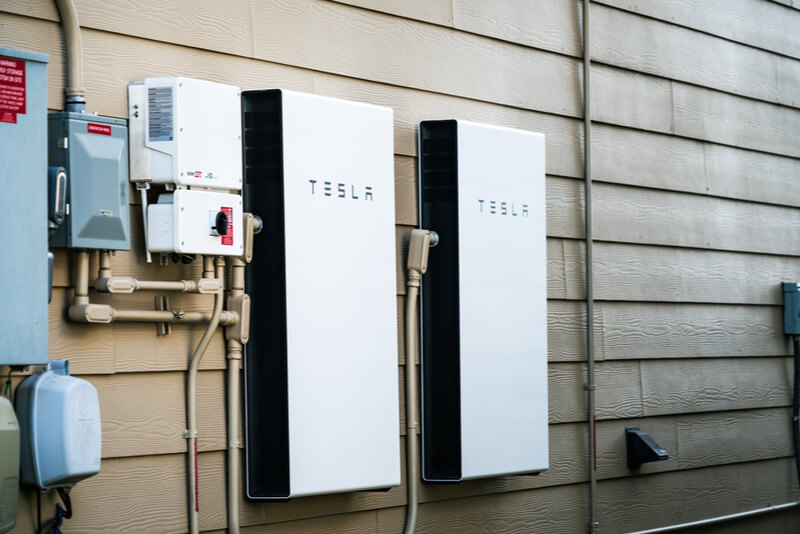
\includegraphics[width=0.4\textwidth]{powerwall}
				\captionsetup{name=Εικόνα}
				\caption{{\latintext{Tesla Powerwall}}.}
				\label{fig:powerwall}
\end{wrapfigure}

Αντίστοιχη χρήση έχει αρχίσει και σε πειραματικό επίπεδο στο εξωτερικό με τις οικιακές μπαταρίες (βλ. {\latintext{Tesla Powerwall}} στην Εικόνα \ref{fig:powerwall}). 
Αυτές αρχικά μπορούν να χρησιμοποιηθούν για ασφάλεια σε περιοχές με συχνές διακοπές ρεύματος, με το να αποθηκεύουν
ηλεκτρική ενέργεια από το δίκτυο και να τροφοδοτούν το σπίτι σε περίπτωση διακοπής. Υπάρχει η λειτουργία μάλιστα να προγραμματιστεί η μπαταρία να απορροφάει ενέργεια από το δίκτυο μόνο τις ώρες με φθηνότερο κόστος (π.χ. νυχτερινό
ρεύμα). Η πραγματική αξία όμως αυτών των τεχνολογιών εμφανίζεται όταν συνδυαστούν με ΑΠΕ. Όση παραγωγή ενέργειας δεν αξιοποιείται επιτόπου, αποθηκεύεται στις μπαταρίες, από τις οποίες ο χρήστης αντλεί ενέργεια για τις βραδυνές
τους καταναλώσεις. Με την χρήση των έξυπνων δικτύων που προαναφέρθηκαν, ο παραγωγός και ο καταναλωτής μπορούν να έχουν αμοιβαίο κέρδος.
Το δίκτυο κάνει ανοιχτή πρόσκληση σε όποιον ενδιαφερόμενο, ώστε να μπορεί να του αντλεί ενέργεια από τις μπαταρίες του, συγκεκριμένες περιόδους του χρόνου (π.χ. Ιούλιος-Σεπτέμβριος που υπάρχει η μέγιστη ζήτηση). Κάθε περισταστικό
διαρκεί κάποιες ώρες (συνήθως τις μεσημεριανές), ενώ υπάρχει όριο στα πόσα περιστατικά θα μπορεί να υπάρξουν στον ενδιαφερόμενο μέσα σε αυτήν την περίοδο (π.χ. 50). Στη συνέχεια το δίκτυο είναι υπεύθυνο να πληρώσει το ποσό 
που έχει εγγυηθεί, το οποίο είναι αρκετά ικανοποιητικό. Με αυτό το ποσό όμως κερδίζουν και οι δύο πλευρές. Το κόστος που θα είχε να λειτουργήσει μία παραπάνω μονάδα παραγωγής ηλεκρικής ενέργειας, 
μόνο για αυτά τα συγκεκριμένα περιστατικά μέσα στην περίοδο, είναι κατά πολύ μεγαλύτερο από την "αγορά" της ενέργειας αυτής από τους ίδιους τους καταναλωτές. Από την άλλη ο καταναλωτής μπορεί να ορίσει το ποσό της ενέργειας
που θα επιτρέπει να δίνει η μπαταρία στο δίκτυο και αν συνδυαστεί αυτό με κάποιο διάστημα που αυτός λείπει από το σπίτι, τότε η ενέργεια που παράγεται από τις ΑΠΕ στο σπίτι του δεν θα πηγαίνει χαμένη καθώς
θα μπορεί να πωλείται ενώ λείπει. Με αυτόν τον τρόπο, αν οι κάτοικοι της περιοχής ενταχθούν σε αυτό το πρόγραμμα, φτιάχνεται μία μεγάλη εικονική μπαταρία για να στηρίζει το δίκτυό της.

Με την ίδια λογική και με τη χρήση των {\latintext{micro-grid}} θα μπορούν ολόκληρες περιοχές να τροφοδοτούνται σε μεγάλο βαθμό μεταξύ τους, μειώνοντας και το ρίσκο διακοπής ρεύματος από τυχόν βλάβη στον κεντρικό παραγωγό. 
Οι κάτοικοι με ΑΠΕ, γεννήτριες, μπαταρίες κ.α. θα υποστηρίζουν το δίκτυο της περιοχής τους, με το αντίστοιχο οικονομικό κέρδος από το δίκτυο. Έτσι βγαίνουν όλοι κερδισμένοι, ακολουθώντας την λογική που αναφέρθηκε
στην προηγούμενη παράγραφο.

Όλα αυτά είναι εξελίξεις, στις οποίες τα έξυπνα δίκτυα μπορούν και θα πρέπει να ανταπεξέλθουν. Η ανθρωπότητα περνάει σε μια εποχή που η χρήση της ενέργειας αλλάζει μορφή, γίνεται αμφίδρομη με στόχο την αποδοτικότητα
και την οικολογία.
\chapter{Παραγωγή Ενέργειας}
\section{Κυψέλες Καυσίμου}
Η κυψέλη καυσίμου είναι μία τεχνολογία που ήδη αξιοποιείται από τη δεκαετία του 60', στα διαστημικά προγράμματα της {\latintext{NASA}}. Η αρχή λειτουργίας της είναι παρόμοια με αυτήν της μπαταρίας. Μία άνοδος και μία κάθοδος
διαχωρίζονται μεταξύ τους από έναν ηλεκτρολύτη. Η άνοδος τροφοδοτείται από μόρια υδρογόνου, ενώ η κάθοδος από οξυγόνου. Κατά την τροφοδοσία της ανόδου, ένας καταλύτης (συνήθως λευκόχρυσος) διαχωρίζει τα μόρια υδρογόνου, 
σε κατιόντα υδρογόνου ({\latintext{\ce{H^+}}}) και ηλεκτρόνια ({\latintext{\(e^-\)}}).
Διαμέσου όμως του ηλεκτρολύτη μπορούν να περάσουν μόνο θετικά φορτισμένα σωματίδια, συνεπώς τα κατιόντα υδρογόνου περνάνε, αλλά τα ηλεκτρόνια πρέπει να ακολουθήσουν διαφορετική διαδρομή. Αυτή η διαδρομή αποτελεί
το κύκλωμα που θα τροφοδοτηθεί από την κυψέλη καυσίμου, συνεπώς εκεί συνδέεται το φορτίο. Από τη στιγμή που τα ηλεκτρόνια ακολουθούν μία σταθερή κατεύθυνση, με σκοπό να καταλήξουν στην πλευρά της καθόδου, το ρεύμα που 
παράγεται είναι συνεχές. Αφού τα ηλεκτρόνια τροφοδοτήσουν το φορτίο, καταλήγουν στην κάθοδο, όπου ενώνονται με τα κατιόντα υδρογόνου ξανά και στη συνέχεια τα μόρια υδρογόνου ενώνονται με το οξυγόνο. 
Συνεπώς το μόνο προϊόν της αντίδρασης είναι το νερό και κάποια ποσά θερμότητας. Για τον λόγο αυτό, η
τεχνολογία των κυψελών καυσίμου χαρακτηρίζεται μηδενικών εκπομπών ({\latintext{zero-emission}}), αν η παραγωγή βέβαια του υδρογόνου συνδυαστεί με ΑΠΕ (βλ. κεφ. \ref{chap:hydrogen}).

\begin{figure}
				\center
				{\latintext{\ce{H2 <-> 2 H^+ + 2 e^- \\[10pt]
												1/2O2 + 2 H^+ + 2 e^- <-> H2O \\[10pt]
												H2 + 1/2O2 <-> H2O}}}
				\captionsetup{width=0.8\textwidth}
				\caption{Χημικές αντιδράσεις που λαμβάνουν χώρα σε μία Κυψέλη Καυσίμου.}
				\label{eq:fuelcell}
\end{figure}

Υπάρχουν διάφορες τεχνολογίες κυψελών καυσίμου, οι οποίες χρησιμοποιούν ξεχωριστά υλικά η κάθε μία. Η κάθε τεχνολογία παρουσιάζει διαφορετικά πλεονεκτήματα (π.χ. ισχύς, βάρος κ.α.), αλλά και διαφορετικά κόστη παραγωγής 
και αποδοτικότητα. Η απόδοση των κυψελών καυσίμου είναι αρκετά ικανοποιητική και κυμαίνεται σε γενικές γραμμές μεταξύ 40-60\%, ενώ αν η κατασκευή τους περιλαμβάνει και την αξιοποίηση της παραγώμενης από αυτές θερμότητας, τότε η 
απόδοση μπορεί να φτάσει μέχρι και τα 80\%. Οι ηλεκτρολύτες μπορεί να είναι είτε στερεοί, είτε υγροί, με τους πρώτους να αποτελούν την πιο μοντέρνα λύση (π.χ. {\latintext{Proton Exchange Membrane Fuel Cell-PEMFC}}). Σύμφωνα με
τους \textcite{diaz2016}:

{\textit{'Ανάλογα με το μέγεθος του συστήματος, μπορούν να χρησιμοποιηθούν διαφορετικά μεγέθη κυψελών καυσίμου. Για παράδειγμα η τεχνολογία {\latintext{PEMFC}}, η οποία και είναι η πιο διαδεδομένη τεχνολογία κυψελών καυσίμου,
λειτουργεί στους {\latintext{\ce{80^oC}}} και προτιμάται για βιομηχανικές εφαρμογές, καθώς στοιβάδες των {\latintext{100kW}}, μπορούν εύκολα να βρεθούν στο εμπόριο. Για εφαρμογές υψηλών ισχύων (της τάξης των {\latintext{MW}}),
η επικαλούμενη {\latintext{Solid Oxide Fuel Cell (SOFC)}}, η οποία λειτουργεί στους {\latintext{\ce{650^oC}}}, είναι καλή επιλογή, διότι μπορεί να βρεθεί εύκολα στο εμπόριο σε στοιβάδες των {\latintext{2MW}}.'}}

\chapter{Αποθήκευση Ενέργειας}
\label{chap:storage}
Η αποθήκευση ενέργειας δεν είναι μία καινούργια ανησυχία. Ανέκαθεν ο άνθρωπος αναζητούσε τρόπους να δεσμεύσει ενέργεια για μελλοντική χρήση, απλά τώρα υπάρχει η κατάλληλη τεχνολογία. 
Με την μεταστροφή σε ένα πιο πράσινο μέλλον έχουν αναπτυχθεί πολλές διαφορετικές τεχνολογίες που εξυπηρετούν ξεχωριστούς σκοπούς, όσον αφορά την αποθήκευση. Οι κύριες τεχνολογίες και οι χρήσεις τους που απασχολούν
τον επιστημονικό τομέα
είναι οι μπαταρίες (κυρίως Λιθίου-Ιόντος) για τα φορτία αιχμής του δικτύου και το υδρογόνο για μακροβιότερες αποθηκεύσεις. Παρ'όλα αυτά δεν θα πρέπει να λησμονείτε η αξιόπιστη αντλησιοταμίευση από αυτές τις τεχνολογίες. 
Στο κεφάλαιο αυτό θα αναφερθούν συνοπτικά αυτές οι κύριες τεχνολογίες αποθήκευσης που απασχολούν τον ενεργειακό τομέα, των οποίων η χρήση δεν είναι απλά επιστημονικά ενδιαφέρουσα, αλλά και οικονομικά συμφέρουσα.

\begin{figure}[h]
				\center
				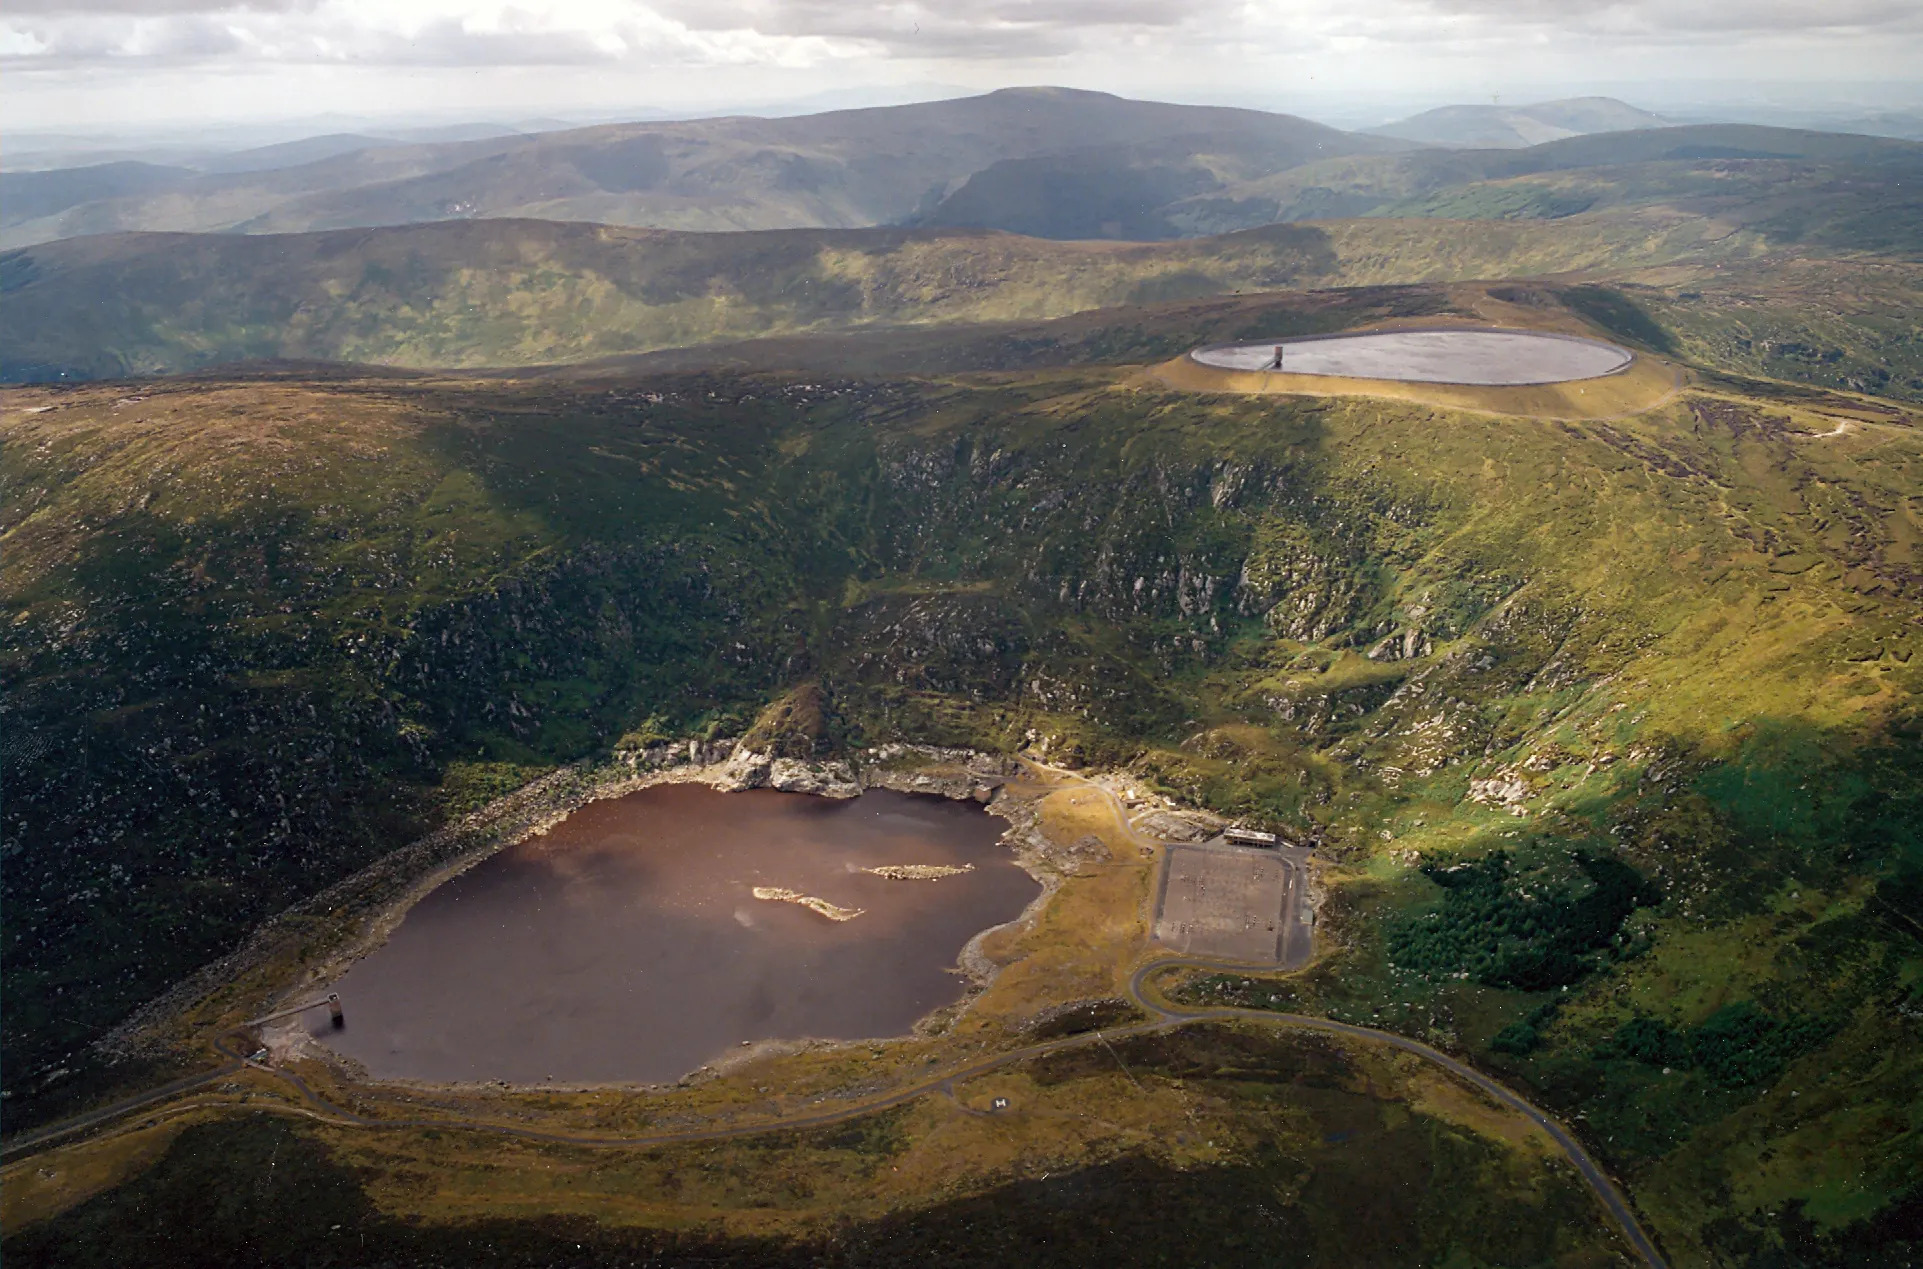
\includegraphics[width=0.7\textwidth]{turlough-hill}
				\captionsetup{name=Εικόνα, width=0.8\textwidth}
				\caption{Το μοναδικό έργο αντλησιοταμίευσης που έχει η Ιρλανδία, στο {\latintext{Turlough Hill}}.}
				\label{fig:turlough-hill}
\end{figure}

\section{Αντλησιοταμίευση}
Τα έργα αντλησιοταμίευσης έχουν εφαρμοσθεί εδώ και πάνω από έναν αιώνα, ώστε να δεσμεύουν την παραπανήσια ενέργεια και να την διαθέτουν στο δίκτυο κατά τις ώρες υψηλής ζήτησης. 
Σύμφωνα με το υπουργείο ενέργειας των ΗΠΑ \parencite{energygov1801}, η πρώτη γνωστή χρήση των έργων αντλησιοταμίευσης ήταν στην Ιταλία και την Ελβετία την δεκαετία το 1890. Οι ίδιες οι ΗΠΑ διαθέτουν 43 τέτοιες μονάδες, οι
οποίες είναι υπεύθυνες μέχρι και σήμερα για το 93\% της ολικής αποθήκευσης ενέργειας του δικτύου τους. 

Προφανώς τα έργα αυτά τότε δεν είχαν γίνει για να καλύψουν το τεχνικό πρόβλημα των ΑΠΕ, αλλά διότι δεν ήταν εφικτό να
σταματάει η λειτουργία των μηχανών, όποτε ελαττωνόταν η ζήτηση. Τα έργα αυτά αποτελούσαν έναν απλό τρόπο να διατηρείται η λειτουργία των μηχανών σε ένα σταθερό επίπεδο, βοηθώντας τες και σε περιπτώσεις αυξημένης κατανάλωσης.
Αντίστοιχα σήμερα, τα έργα αυτά παίζουν καθοριστικό ρόλο στην ένταξη των ΑΠΕ στο δίκτυο ηλεκτρικής ενέργειας, καθώς η τεχνολογία και οι εγκαταστάσης επιβιώνουν μέχρι και σήμερα, χωρίς να έχει σταματήσει η λειτουργία τους.

Η λειτουργία των συστημάτων αυτών είναι αρκετά απλή στη σύλληψη και βασίζεται κατά κύριο λόγο στη βαρυτική δύναμη. Είτε κατασκευάζονται, είτε υπάρχουν φυσικά, υπάρχουν δύο δεξαμενές σε διαφορετικό υψόμετρο η μία από την άλλη.
Κατά την διάρκεια την οποία υπάρχει πλεόνασμα ενέργειας στο δίκτυο, η ενέργεια αυτή χρησιμοποιείται για να ξεκινήσουν οι αντλίες να γεμίζουν την πάνω δεξαμενή, με το νερό της κάτω. Όταν πια χρειαστεί να υπάρξει έκχυση 
ηλεκτρικής ενέργειας στο δίκτυο, το αποθηκευμένο νερό της πάνω δεξαμενής, αφήνεται να κυλισει προς την κάτω. Κατά τη διαδρομή του, το νερό συναντάει υδροστροβίλους, οι οποίοι με την περιστροφική τους κίνηση μπορούν
να διαθέσουν την ισχύ τους στο δίκτυο. 

Η αντλησιοταμίευση παρουσιάζει πολλά θετικά και δικαιολογημένα αποτελεί την πλέον αξιόπιστη και δοκιμασμένη λύση στον τομέα της μαζικής αποθήκευσης ενέργειας. Αρχικά παρουσιάζει πολύ μεγάλη απόδοση της τάξης των 80\%, 
ενώ το όριο ζωής της είναι τα 50 χρόνια. Αυτά συνδυάζονται με την προαναφερθήσα απλή λειτουργία και συντήρηση του έργου.

Παρ'όλα αυτά θα πρέπει να τονιστούν κάποιες δυσκολίες. Η εύρεση ενός κατάλληλου μορφολογικά εδάφους, δεν είναι κάτι εύκολο. Θα πρέπει να υπάρχει τουλάχιστον 100{\latintext{m}} υψομετρική διαφορά μεταξύ της μίας δεξαμενής 
από την άλλη, για να έχει νόημα οποιαδήποτε επένδυση, ενώ παράλληλα αυτές οι δεξαμενές δεν θα πρέπει να είναι και πολύ μακριά μεταξύ τους. Αυτό σημαίνει ότι συνήθως συναντάμε κατάλληλες μορφολογίες σε ιδιαίτερα δύσβατα μέρη, 
κάτι που μπορεί να καθιστά την κατασκευή πολύ δαπανηρή, ίσως και ασύμφορη. Επιπλέον, για τον ίδιο λόγο, μπορεί η περιοχή να μην παρέχει πρόσβαση στο δίκτυο ηλεκτρικής ενέργειας, συνεπώς η σύνδεση του έργου με το δίκτυο να είναι 
ανέφικτη. Τέλος η κατασκευή του έργου είναι δαπανηρή, ενώ δεν θα πρέπει να παραβλέπονται οι πιθανές περιβαλλοντικές επιπτώσεις στα οικοσυστήματα της περιοχής.

Στην πράξη όμως τα έργα αντλησιοταμίευσης έχουν αποδείξει την αξία τους και δεν κατέχουν τυχαία την κυρίαρχη θέση στην αποθήκευση, καθώς με την απλή τους κατασκευή και λειτουργία, 
κατατάσσονται στα μακροβιότερα και πιο αξιόπιστα συστήματα αποθήκευσης ηλεκτρικής ενέργειας. Έργα πολλών δεκαετιών συνεχίζουν να λειτουργούν εξίσου καλά μέχρι και σήμερα, ενώ παρόλο τον ανταγωνισμό των νέων τεχνολογιών,
παραμένουν η καλύτερη λύση όσον αφορά την μακρυχρόνια αποθήκευση.
\section{Συσσωρευτές}
Στην έννοια της μπαταρίας περιλαμβάνεται ένα πολύ ευρύ φάσμα διαφορετικών τεχνολογίων, οι οποίες παρ'όλο που ακολουθούν μία κοινή αρχή λειτουργίας, η απόκρισή τους σε διαφορετικές συνθήκες χρήσης διαφέρει σε μεγάλο βαθμό. 
Οι παράγοντες που επηρεάζουν την συμπεριφορά των συσσωρευτών είναι τόσοι πολλοί, που μέχρι και σήμερα η μοντελοποίησή τους είναι μία πολύπλοκη διαδικασία. Μέσα στα χρόνια έχουν αναπτυχθεί πολλές τεχνολογίες μπαταρίας, 
αλλά στη σημερινή εποχή και συγκεκριμένα στον τομέα της ενέργειας, οι δύο μεγάλοι συναγωνιστές είναι οι μπαταρίες Μολύβδου-Οξέος και οι μπαταρίες Λιθίου-Ιόντος.
\subsection{Αρχή Λειτουργίας}
Σε αυτό το κεφάλαιο αναλύεται η αρχή λειτουργίας της μπαταρίας Μολύβδου-Οξέος, αλλά με βάση αυτήν, μπορεί να γίνει κατανοητή η λειτουργία οποιουδήποτε συσσωρευτή. 

Η καρδιά της μπαταρίας είναι η πλάκα ή αλλιώς ηλεκτρόδιο.
Η πλάκα δομείται από ένα δικτύωμα, το οποίο είναι επικαλυμμένο με διοξείδιο του μολύβδου ({\latintext{\ce{PbO2}}}), σε συνδυασμό και με άλλα πρόσθετα, τα οποία συμβάλλουν στην αντοχή της πλάκας και την αντίστασή της στη διάβρωση. 
Το συγκεκριμένο ηλεκτρόδιο αποτελεί τον αρνητικό πόλο της μπαταρίας (άνοδος). Αντίστοιχη πλάκα υπάρχει και για τον θετικό πόλο της μπαταρίας (κάθοδος), 
αλλά σε αυτήν την περίπτωση είναι επικαλυμμένος με καθαρό μόλυβδο ({\latintext{\ce{Pb}}}). Αυτές οι πλάκες δεν πρέπει να 
έρθουν σε επαφή μεταξύ τους, διότι θα προκληθεί βραχυκύκλωμα. Συνεπώς τοποθετείται η άνοδος μέσα σε έναν πορώδη "φάκελο". 
Τέλος ο υπόλοιπος χώρος ανάμεσα στις πλάκες πληρώνεται με έναν ηλεκτρολύτη, αποτελούμενος από νερό ({\latintext{\ce{H2O}}}) και θειικό οξύ ({\latintext{\ce{H2SO4}}}).

Η πρώτη αντίδραση που λαμβάνει χώρα σε αυτό το σύστημα είναι η ένωση των θειικών του ηλεκτρολύτη με τον μόλυβδο, δημιουργώντας με αυτόν τον τρόπο μία επίστρωση θειικού μολύβδου ({\latintext{\ce{PbSO4}}}) και στις δύο πλάκες. 
Κατά την αντίδραση αυτή, η άνοδος με την προσρόφηση ηλεκτρονίων, απελευθερώνει τα άτομα οξυγόνου από το διοξείδιο του μολύδου, τα οποία ενώνονται με τα ιόντα υδρογόνου του ηλεκτρολύτη, δημιουργώντας νερό. Από την άλλη στην κάθοδο,
η αντίδραση ελευθερώνει δύο ηλεκτρόνια, τα οποία μην έχοντας τρόπο να φτάσουν στην άνοδο μέσω του ηλεκτρολύτη\footnote{Οι ηλεκτρολύτες είναι ουσίες που επιτρέπουν την κίνηση ιόντων, αλλά όχι ηλεκτρονίων. Τα οποιαδήποτε ρεύματα
υπάρχουν σε ένα τέτοιο διάλυμα, οφείλονται αποκλειστικά στην κίνηση των ιόντων αυτών.}, συσσωρεύονται στην κάθοδο. Όταν πια εξαντληθούν τα διαθέσιμα ηλεκτρόνια, ώστε να λάβουν χώρα οι αναγκαίες αντιδράσεις, το σύστημα φτάνει σε
μία ισορροπία. Την στιγμή όμως, που ένα εξωτερικό κύκλωμα ενώσει την κάθοδο με την άνοδο, τα συσσωρευμένα ηλεκτρόνια βρίσκουν δίοδο διαμέσου αυτού και οι αντιδράσεις μπορούν να συνεχιστούν. Από τη στιγμή που τα ηλεκτρόνια ακολουθούν
την συγκεκριμένη κατεύθυνση αυτή, συμπεραίνει κανείς ότι το ρεύμα που προσδίδουν οι μπαταρίες είναι συνεχές.

\begin{figure}[h]
				\center
				{\latintext{\ce{Pb + H2SO4 <-->[Discharge][Charge] PbSO4 + 2 e^- \\[14pt]
												PbO2 + H2SO4 + 2 e^- <-->[{Discharge}][{Charge}] PbSO4 + 2 H2O \\[14pt] 
												PbO2 + 2 H2SO4 + Pb <-->[{Discharge}][{Charge}] 2 PbSO4 + 2 H2O}}}
				\captionsetup{width=0.8\textwidth}
				\caption{Χημικές αντιδράσεις καθόδου, ανόδου και ολικά.}
				\label{eq:battery}
\end{figure}

Αυτό όμως δεν μπορεί να γίνει επ'άπειρον, διότι καθώς ο ηλεκτρολύτης αραιώνεται με την δημιουργία νερού, τα χημικά στοιχεία τα οποία είναι αναγκαία για αυτές τις μετατροπές, όλο και μειώνονται. 
Επίσης, αυξάνεται η επίστρωση του θειικού μολύβδου και στις δύο πλάκες, με αποτέλεσμα τα ηλεκτρόδια να γίνονται παρόμοιας σύστασης, μειώνοντας την τάση που έχουν τα χημικά στοιχεία να αντιδράσουν μεταξύ τους. 
Παρ'όλα αυτά είναι εφικτή η αντιστροφή των προηγουμένων αντιδράσεων, με στόχο την επαναφορά της μπαταρίας στην αρχική της κατάσταση, δηλαδή την φόρτισή της. 
Αυτό γίνεται με την εξαναγκασμένη αντιστροφή της ροής των ηλεκτρονίων, διαμέσου του ίδιου αγωγού και συνεπώς της εξαναγκασμένης αντιστροφής των χημικών διεργασιών. 

Όταν μία μπαταρία ξεφωρτίζεται σε μεγάλα βάθη, οι επιστρώσεις του θειικού μολύβδου πάνω στις πλάκες, αυξάνονται σε τέτοιο βαθμό, όπου το βάρος τους υπερνικάει την προσκόλλησή τους και κατακάθονται σαν ίζημα στον πυθμένα του κελύφους
του συσσωρευτή. Με αυτόν τον τρόπο, κάποια από τα χημικά στοιχεία που ήταν αναγκαία για τις αντιδράσεις, δεν λαμβάνουν μέρος πια σε αυτές, μειώνοντας έτσι την αποθηκευτική ικανότητα της μπαταρίας.

Όλο αυτό το σύστημα που περιγράφθηκε παραπάνω αποτελεί μία κυψέλη. Η διαφορά δυναμικού μεταξύ των δύο ηλεκτροδίων της κυψέλης, καθορίζεται από τα χημικά στοιχεία που χρησιμοποιούνται στον συγκεκριμένο τύπο συσσωρευτή και όχι
από το μέγεθός της. 
Συγκεκριμένα για τις μπαταρίες Μολύβδου-Οξέος, η τάση κυψέλης ανέρχεται στα {\latintext{2-2.1V}} (για τις τιμές των υπολοίπων συσσωρευτών βλ. Πίνακα \ref{tab:battery}). Το μέγεθος των πλακών της μπαταρίας καθορίζει 
την αγωγιμότητα, συνεπώς και το ρεύμα που μπορεί να παροχετευτεί στο εξωτερικό κύκλωμα. Αυτός είναι και ο λόγος που οι μπαταρίες είναι συγκεκριμένης τάσης, αλλά διαφορετικών φορτίων ({\latintext{Ah}}). 
Τα {\latintext{2V}} όμως, της μίας κυψέλης, δεν είναι ικανά να τροφοδοτήσουν σχεδόν καμία καθημερινή συσκευή. Για να φτάσουν οι μπαταρίες μία ικανοποιητική τάση εξόδου, συνδέονται σε σειρά έξι τέτοιες κυψέλες, 
φτάνοντας με αυτόν τον τρόπο τα συνήθη {\latintext{12V}}, που βρίσκονται για παράδειγμα στις περισσότερες μπαταρίες αυτοκινήτου, ενώ αν υπάρξουν και παράλληλες συνδέσεις, μπορούν να επιτευχθούν και οι επιθυμητές τιμές των ρευμάτων.

\begin{table}[h]
\centering
				\begin{tabular}{ |c|c| }
				\hline
				Tύπος Μπαταρίας & Ονομαστική Τάση Κυψέλης ({\latintext{V}}) \\
				\hline
				Μολύβδου-Οξέος & 2 \\
				Λιθίου-Ιόντος & 3.6 \\
				Νικελίου-Καδμίου & 1.2 \\
				\hline
				\end{tabular}
\captionsetup{width=0.8\textwidth}
\caption{Ονομαστικές τάσεις κυψέλης για τους τρεις πιο διαδεδομένους τύπους μπαταριών.}
\label{tab:battery}
\end{table}

\subsection{Ιδιαιτερότητες Συσσωρευτών}
Οι μπαταρίες χαρακτηρίζονται από γρήγορη απόκριση\footnote{Γι'αυτό και χρησιμοποιούνται και στις γεννήτριες (ΗΖ) σε περιπτώσεις διακοπής ρεύματος. Τα ΗΖ χρειάζονται κάποια κρίσιμα δευτερόλεπτα για να φτάσουν πλήρη λειτουργία, τα
οποία δεν είναι πάντα εφικτό να υπάρξουν. Σε εγκαταστάσεις ειδικά που υπάρχουν εξειδικευμένα μηχανήματα και υπολογιστές, αυτή η διακοπή στη λειτουργία τους μπορεί να προκαλέσει μόνιμη βλάβη. Οι μπαταρίες με την γρήγορη
απόκρισή τους μπορούν να λειτουργήσουν σαν μεσάζοντας μεταξύ δικτύου και της εφεδρικής γεννήτριας, διασφαλίζοντας μία σίγουρη μετάβαση μεταξύ των δύο.} και μεγάλη απόδοση. Παρ'όλα αυτά χρήζουν ιδιαίτερα προσεκτικής μεταχείρησης, 
καθώς δεν είναι λίγοι οι παράγοντες που μπορούν να προκαλέσουν την μόνιμη υποβάθμισή της.

Αρχικά για τις μπαταρίες Μολύβδου-Οξέος, η θερμοκρασία μπορεί να μειώσει σε μεγάλο βαθμό την απόδοση μιας μπαταρίας. Σε χαμηλές θερμοκρασίες μειώνεται η τάση και η χωρητικότητα του συσσωρευτή, 
ενώ σε υψηλές μειώνεται αισθητά η διάρκεια ζωής του. Συγκεκριμένα 
η διάρκεια ζωής της μπαταρίας μειώνεται κατά 50\% για κάθε {\latintext{\ce{10^oC}}}, πάνω από τη βέλτιστη θερμοκρασία λειτουργίας των {\latintext{\ce{25^oC}}}. Σε αυτήν την βέλτιστη θερμοκρασία λειτουργίας, παρουσιάζεται
μία αυτοεκφόρτιση της μπαταρίας, με ρυθμό 1-5\% μηνιαίως.

Οι μπαταρίες Μολύβδου-Οξέος ακόμα αποτελούν την προτιμητέα λύση, όσον αφορά τα συστήματα ΑΠΕ, διότι διατηρούν την τιμή τους σε πολύ χαμηλά επίπεδα. Αυτό όμως αντισταθμίζεται με την τακτική συντήρηση που χρειάζονται. 
Το υγρό του ηλεκτρολύτη θα πρέπει να αλλάζεται ανά τακτικά χρονικά διαστήματα, με σκοπό την αναπλήρωση των χαμένων χημικών ουσιών. Θα πρέπει να δίνεται μεγάλη προσοχή επίσης στον χώρο που θα τοποθετούνται οι συσσωρευτές αυτοί.
Σε πολύ κρύες τοποθεσίες το νερό στον ηλεκτρολύτη μπορεί να παγώσει και να διογκωθεί, προκαλώντας ρωγμές και καταστρέφοντας την δομή της μπαταρίας. Επίσης κατά τη λειτουργία της μπαταρίας και σε υψηλές θερμοκρασίες, μπορεί να
παραχθούν βλαβερά αέρια, τα οποία θα πρέπει να απομακρύνονται από τους κλειστούς χώρους, μέσω ενός κατάλληλα διαμορφωμένου συστήματος απαγωγής αερίων.
 
Υπάρχουν βέβαια συσσωρευτές Μολύβδου-Οξέος που δεν απαιτούν τόση τακτική συντήρηση, διότι ο υγρός ηλεκτρολύτης έχει αντικατασταθεί από έναν στερεού τύπου ({\latintext{Gel}}). Το πρόβλημα έγκειται στην αυξημένη τιμή τους, αλλά
και στην μικρότερη διάρκεια ζωής τους. 

Οι μπαταρίες Λιθίου-Ιόντου δεν παρουσιάζουν τις ίδιες συμπεριφορές στις καιρικές συνθήκες και στις διαφορετικές μεταχειρίσεις. Επιδεικνύουν μία μεγαλύτερη αντοχή σε αυτές, όχι όμως ότι στερούνται ιδιοτροπιών. 
Δεν θα πρέπει αρχικά αυτές οι μπαταρίες να υπερφορτίζονται ή να φορτίζονται σε χαμηλές θερμοκρασίες, κάτι που σημαίνει ότι τα συστήματα που περιλαμβάνουν τέτοιου τύπου συσσωρευτές, θα πρέπει να συνδυάζονται με συστήματα
διαχείρισης συσσωρευτών ανά στοιχείο {\latintext{(Battery Management System-BMS)}}. Το σημαντικότερο μειονέκτημά τους όμως είναι το υψηλότερο κόστος και ότι υπάρχει πιθανότητα να περιέχουν τοξικές ουσίες, όπως το κοβάλτιο.

Από την άλλη, οι συσσωρευτές Λιθίου-Ιόντου έχουν υψηλή ενεργειακή πυκνότητα και γι'αυτό είναι μονόδρομος πια σε μικρές ηλεκτρικές συσκευές. Επίσης έχουν μεγάλο βάθος εκφόρτισης {\latintext{(Depth of Discharge-DoD)}}, που μπορεί
να φτάσει μέχρι και το 100\%. Όλα αυτά συνδυάζονται με υψηλή διάρκεια ζωής, μηδενική ανάγκη συντήρησης, ικανότητα σταθερής λειτουργίας σε μεγάλο εύρος θερμοκρασιών και χαμηλή αυτοεκφόρτιση.

Κάθε τύπος μπαταρίας έχει διαφορετικές τάσεις φόρτισης, διαφορετικά βάθη εκφόρτισης και γενικότερα ξεχωριστά τεχνικά χαρακτηριστικά. Συνεπώς η χρήση ενός είδους συσσωρευτή προϋποθέτει την σωστή μελέτη της συμπεριφοράς του.
Σε γενικές γραμμές, όλοι οι τύποι μπαταριών παρουσιάζουν μη-γραμμική συμπεριφορά, δηλαδή το διαθέσιμο περιεχόμενό τους δεν είναι σταθερό, αλλά διαφέρει με βάση τις προαναφερθείσες παραμέτρους.

\section{Υδρογόνο}
\label{chap:hydrogen} 
Το υδρογόνο χρησιμοποιείται εδώ και χρόνια στην διαστημική τεχνολογία, καθώς αποτελεί το κύριο προωθητικό καύσιμο για τους πυραύλους. Σε αντίθεση με τα υπόλοιπα καύσιμα, το υδρογόνο δεν είναι ανθρακούχος ύλη. 
Η χρήση του περιλαμβάνει κυρίως δύο τρόπους, είτε την άμεση καύση του, 
είτε την μετατροπή του σε ηλεκτρική ενέργεια, μέσω κυψελών καυσίμου. Και στις δύο περιπτώσεις το υδρογόνο οξειδώνεται και το μόνο παραπροϊόν της αντίδρασης είναι το νερό. 
Στην πρώτη περίπτωση, η θερμότητα που παράγεται χρησιμοποιείται για την κίνηση συμβατικών μηχανών εσωτερικής καύσης (ΜΕΚ), ενώ στη δεύτερη περίπτωση το ηλεκτρόνια από την αντίδραση των παραπάνω στοιχείων 
προμηθεύουν τους κινητήρες με ηλεκτρική ενέργεια.

Ενώ όμως το υδρογόνο είναι από τα πιο άφθονα στοιχεία στον κόσμο, δεν μπορεί να βρεθεί εύκολα στην ατομική του μορφή, παρά μόνο σε μοριακές ενώσεις. Η διαδικασία της εξαγωγής του υδρογόνου από τα μόρια αυτά, 
καθορίζει σε τελικό βαθμό, το κατά πόσο η τεχνολογία αυτή είναι φιλική προς το περιβάλλον ή όχι. Μέχρι και σήμερα οι δύο βασικοί τρόποι εξαγωγής του υδρογόνου είναι η αναμόρφωση του μεθανίου ({\latintext{\ce{CH_4}}}) και η
ηλεκτρόλυση του νερού.

Η πρώτη μέθοδος είναι η πιο διαδεδομένη μορφή μαζικής παραγωγής υδρογόνου. Η διαδικασία βασίζεται στο ότι το μεθάνιο μπορεί να διασπαστεί σε μονοξείδιο του άνθρακα και υδρογόνο, όταν έρθει σε επαφή με υψηλής 
θερμοκρασίας υδρατμούς (Σχήμα \ref{eq:reform}). Αλλά ενώ το τελικό προϊόν είναι μηδενικών εκπομπών, όλη η διαδικασία αυτή χρειάζεται τρομερά ποσά θερμότητας, το οποίο την καθιστά υπερβολικά αντιαποδοτική και 
περιβαλλοντικά προβληματική. Συνήθως το μεθάνιο από αυτήν τη διαδικασία προσλαμβάνεται από την επεξεργασία και αεριοποίηση βιομάζας, κάνοντας όλην την διαδικασία πιο "πράσινη".

\begin{figure}[h]
				\center
				{\latintext{\ce{CH4 + H2O ->[heat] CO + 3 H2}}}
				\caption{Χημική αντίδραση Αναμόρφωσης Μεθανίου.}
				\label{eq:reform}
\end{figure}

Η ηλεκτρόλυση από την άλλη βασίζεται στη διάσπαση του νερού σε υδρογόνο και οξυγόνο, όταν αυτό διαπερνάται από υψηλά ποσά ηλεκτρικού ρεύματος \ref{eq:electrolysis}. Η τελική ενέργεια που χρειάζεται να δαπανηθεί είναι
μεγαλύτερη από αυτήν της αναμόρφωσης του μεθανίου, αλλά η τεχνική αυτή βασίζεται στο ότι η ηλεκτρική ενέργεια για τη διάσπαση παράγεται από ανανεώσιμες πηγές ενέργειας. 

\begin{figure}[h]
				\center
				{\latintext{\ce{2 e^- + 2 H2O -> H2 + 2 OH^-}}}
				\caption{Ηλεκτρόλυση Νερού.}
				\label{eq:electrolysis}
\end{figure}

Σε αντίθεση με τις μπαταρίες, το υδρογόνο έχει πολύ μεγάλη ενεργειακή πυκνότητα.
Συγκεκριμένα η ενεργειακή πυκνότητα του συμπιεσμένου υδρογόνου είναι γύρω στις 40,000{\latintext{Wh/kg}}, σε αντίθεση με τις μπαταρίες Λιθίου-Ιόντος που είναι λιγότερο από 280{\latintext{Wh/kg}}. Αυτό είναι 
πολύ σημαντικό για τον τομέα των μεταφορών, καθώς το μεγάλο πρόβλημα της ηλεκτροκίνησης είναι η μικρή αυτονομία. Ένα όχημα που κινείται με υδρογόνο θα μπορεί να διανύει μεγάλες αποστάσεις, κρατώντας το βάρος του σε λογικά επίπεδα.
Ειδικά για τα πλοία, τα φορτηγά, αλλά κυρίως για τα αεροπλάνα, που δεν μπορούν να μεταφέρουν το βάρος τόσων συσσωρευτών που χρειάζεται η κίνησή τους, το υδρογόνο θα μπορούσε να είναι μία εφικτή λύση στο ενεργειακό τους πρόβλημα. 
Δεν πρέπει να ξεχνιέται ούτως ή άλλως, ότι τα παραπάνω μεταφορικά μέσα, αποτελούν ένα μεγάλο μέρος των εκπομπών βλαβερών ουσιών για το περιβάλλον. Το υδρογόνο είναι μία λύση την οποία αναλύουν πολλές κατασκευάστριες εταιρίες 
οχημάτων και για τον λόγο του εφοδιασμού. Το υδρογόνο χρειάζεται λιγότερο από 5 λεπτά για τον πλήρη ανεφοδιασμό του, σε αντίθεση με τις μπαταρίες, που για να φορτίσουν μπορεί να χρειαστούν μέχρι και μερικές ώρες. 

Το σημαντικό πρόβλημα με το υδρογόνο είναι η μεταφορά του και η διανομή του. Σε αντίθεση με τις υφιστάμενες εγκαταστάσεις διανομής ηλεκτρικής ενέργειας, το κόστος για την συμπίεση, μεταφορά και διανομή του υδρογόνου είναι μεγάλο.
Το υδρογόνο παρ'όλο που όπως προαναφέρθηκε διαθέτει υψηλή ενεργειακή πυκνότητα, το ίδιο το στοιχείο είναι πολύ μικρής πυκνότητας. Αυτό σημαίνει ότι για ένα δεδομένο βάρος υδρογόνου, ο όγκος που καταλαμβάνει είναι τεράστιος.
Για να είναι συνεπώς εύκολη η χρήση του πρέπει να συμπιεστεί και αυτό επιτυγχάνεται είτε με την αύξηση της πίεσής του (περίπου στις 700{\latintext{atm}}), είτε με την μείωση της θερμοκρασίας τους κάτω από τους 
{\latintext{\ce{250^oC}}}. Η διαδικασία της ηλεκτρόλυσης όμως, μπορεί να λάβει χώρα {\latintext{in-situ}}, μειώνοντας κατά ένα βαθμό αυτά τα κόστη.

\begin{center}
\pgfornament[width=0.04\textwidth, opacity=0.7]{7}
\end{center}

Αυτό που θα πρέπει να γίνει κατανοητό είναι ότι δεν υπάρχει κάποια τεχνολογία που να λύνει όλο το πρόβλημα της αποθήκευσης. Υπάρχει λόγος που υπάρχουν διαφορετικοί μέθοδοι αποθήκευσης της ενέργειας και ένα σωστό μελλοντικό
πλάνο οφείλει να τις περιλαμβάνει όλες, ανάλογα με το είδος της αποθήκευσης που χρειάζεται. Οι μπαταρίες συμπεριφέρονται πολύ καλά σε γρήγορες απαιτήσεις φορτίου, ενώ υστερούν σε μακροχρόνια αποθήκευση. Αυτό το κενό θα
μπορούσαν να το καλύψουν τα υδροηλεκτρικά έργα, ενώ ένα είδος αποθήκευσης της μορφής του σημερινού καυσίμου που θα μπορούσε να χρησιμοποιηθεί στις μεταφορές θα ήταν το υδρογόνο. Όπως και με την παραγωγή ενέργειας, έτσι και
με την αποθήκευσή της, ένα υπεύθυνο πλάνο για το ενεργειακό μέλλον θα πρέπει να περιλαμβάνει πολλαπλές πηγές παραγωγής και αποθήκευσης, αξιοποιώντας τα θετικά της κάθε μίας, εξαλείφοντας την εξάρτηση μία πηγή, 
δηλαδή των μοναδικών σημείων αποτυχίας ({\latintext{Single Point of Failure - SPOF}}).  
\chapter{Πρόγραμμα}
Σκοπός του προγράμματος είναι να βρεθεί το πλήθος των μπαταρίων που χρειάζονται, για να προστεθούν περισσότερες ΑΠΕ στο δίκτυο. Καθώς τρέχει το πρόγραμμα, εάν συναντήσει μία από τις παρακάτω συνθήκες, τερματίζει.

\begin{enumerate}[label=\roman*]
				\item Όλη η παραγόμενη ενέργεια από τις ΑΠΕ, αξιοποιείται.
				\item Οι ΑΠΕ μαζί με τις μπαταρίες τροφοδοτούν το 100\% του δικτύου.
				\item Το κόστος του συστήματος αποθήκευσης, φτάσει το μέγιστο αποδεκτό από τον χρήστη.
\end{enumerate}

Η τροφοδοσία του δικτύου ολόκληρων περιοχών μόνο από ΑΠΕ και μπαταρίες, απαιτεί τεράστιες χωρητικότητες, τις οποίες οι μπαταρίες των τεχνικών φυλλαδίων δεν έχουν (και δεν χρειάζεται να
έχουν, διότι δεν εξυπηρετούν αυτόν τον σκοπό). Το ίδιο, αλλά προφανώς σε μικρότερο βαθμό, ισχύει και για την αξιοποίηση όλης της παραγώμενης ενέργειας από ΑΠΕ.
Συνεπώς για τους παραπάνω λόγους, η χωρητικότητα της μοναδιαίας μπαταρίας αυξήθηκε, από την τάξη των {\latintext{kWh}} σε αυτήν των {\latintext{MWh}}. Με αυτόν τον τρόπο, η κάθε μία μπαταρία αναπαριστάται
σαν ένα πακέτο χιλίων συσσωρευτών. Συνεπώς, όταν στα αποτελέσματα αναγράφονται 22 μπαταρίες, εννοούνται 22 μπαταρίες με την αυξημένη αυτή χωρητικότητα, δηλαδή 22000 μπαταρίες του αντίστοιχου τύπου, που δίνεται στο τεχνικό φυλλάδιο.
Η παραπάνω θεώρηση προσφέρει και αυξημένη ταχύτητα στο πρόγραμμα, καθώς η διαδικασία της εύρεσης του βέλτιστου πλήθους μπαταριών γίνεται με μεγαλύτερο και πιο ουσιαστικό βήμα. Βέβαια
αν χρειάζεται να αλλαχθεί αυτό και η μοναδιαία μπαταρία πρέπει να έχει τη χωρητικότητα που αναγράφει το τεχνικό φυλλάδιο, απλά τροποποιείται ο αριθμός που αντιπροσωπεύει τη χωρητικότητα
του συσσωρευτή, στα αντίστοιχα αρχεία {\latintext{lead\_carbon.json}} και {\latintext{lithium\_ion.json}}. Σε αυτά τα αρχεία αναγράφονται όλα τα στοιχεία που αντιπροσωπεύουν τις μπαταρίες αυτές.
Το πρόγραμμα αρχικά ζητάει να εισαχθούν κάποιοι, αναγκαίοι για τη λειτουργία του, παράμετροι, οι οποίοι είναι:

\begin{enumerate}[label=\roman*]
				\item Η περιοχή μελέτης.
				\item Ο τύπος μπαταρίας.
				\item Το μέγεθος της ΦΒ εγκατάστασης, που θέλει να έχει περιοχή.
				\item Το όριο κόστους του έργου.
\end{enumerate}

Αφού γίνει αυτό, εισάγονται τα δεδομένα φορτίου της επιλεχθείσας περιοχής, από το αντίστοιχο αρχείο {\latintext{csv}}. Στη συνέχεια, το πρόγραμμα κατεβάζει από την ιστοσελίδα του {\latintext{PV-GIS}}, την ετήσια
παραγωγή του συγκεκριμένου μεγέθους συστήματος, για την υπό εξέταση περιοχή \footnote{Αυτός ο τρόπος καθιστά εύκολη τη μελέτη οποιασδήποτε περιοχής, καθώς το πρόγραμμα χρειάζεται μόνο τη
χρονοσειρά του φορτίου του δικτύου και την αντίστοιχη παραγωγή ΑΠΕ για να λειτουργήσει. Συνεπώς αν υπάρχει το φορτίο δικτύου για μια περιοχή, μπορεί εύκολα να γίνει μελέτη πάνω σε αυτήν, καθώς τα δεδομένα της παραγωγής
των ΦΒ, κατεβάζονται από την ιστοσελίδα, με βάση τις συντεταγμένες της περιοχής.}.
Κατά τη λειτουργία του, το πρόγραμμα χωρίζει το έτος σε ημέρες και για κάθε ημέρα πραγματοποιεί τις ενέργειες που αναφέρονται παρακάτω. Αρχικά αφαιρεί την ισχύς που παράγουν οι ΑΠΕ από την αντίστοιχη καμπύλη φορτίου του δικτύου. 
Αν η παραγώμενη ισχύς των ΑΠΕ είναι παραπάνω από αυτήν του φορτίου, τότε αυτή είναι παραπανήσια και η ημερήσια παραπανήσια ενέργεια, αποθηκεύεται στις μπαταρίες. Στη συνέχεια ξεφορτίζει τις μπαταρίες, για να εξομαλύνει την καμπύλη
φορτίου, ξεκινώντας από τις μεγαλύτερες κορυφές. Αυτό το κάνει μέχρι η μπαταρία να φτάσει στο επιτρεπόμενο βάθος εκφόρτισης που δίνει ο κατασκευαστής. Αφού το κάνει αυτό και διατηρώντας
την στάθμη φόρτισης των μπαταριών, περνάει στην επόμενη μέρα, μέχρι να φτάσει στο τέλος του έτους. ΄Οταν φτάσει στο τέλος του έτους, καταγράφει την ενέργεια που παρήγαγαν οι ΑΠΕ και δεν
μπόρεσε να αποθηκευτεί, την καμπύλη φορτίου του δικτύου, η οποία έχει ελλατωθεί και το κόστος του συστήματος. Αν δεν επιτευχθεί κάποιο από τα αρχικά σενάρια, τότε αυξάνει κατά 1 το μέγεθος
του συστήματος αποθήκευσης και ξαναξεκινάει την ίδια διαδικασία από την αρχη (ουσιαστικά μία {\latintext{nested for loop}}).

Στο τέλος παρουσιάζονται τα αποτελέσματα. Αυτά αναφέρουν το μέγεθος των ΦΒ που ζητήθηκαν και το πλήθος των μπαταριών που επέλεξε το πρόγραμμα ως βέλτιστο, καθώς και τα αντίστοιχα
αρχικά κόστη τους. Επίσης αναγράφονται τα κόστη που έχουν να κάνουν με την λειτουργία, τη συντήρηση, αλλά και τυχόν επαναεπενδύσεις που χρειάζεται να γίνουν, κατά τη διάρκεια ζωής του
έργου (όπως η αγορά καινούργιων μπαταριών, μετά το πέρας της ζωής των προηγουμένων). Δίνεται επίσης μία σημείωση, με το ποια συνθήκη, από αυτές που αναφέρθηκαν αρχικά, επιτεύχθηκε. Πριν
τερματίσει το πρόγραμμα, εμφανίζει μία λίστα με τις παραμέτρους που μπορούν να τροποποιηθούν για να εξατομικευθεί το πρόγραμμα, ανάλογα με τις ανάγκες του κάθε χρήστη. Οι παράμετροι αυτοί
είναι ουσιαστικά μεταβλητές που αρχικοποιούνται στο αρχείο {\latintext{config.py}} και περιλαμβάνουν:

\begin{enumerate}[label=\roman*]
				\item Το εύρος των μπαταριών που ψάχνει το πρόγραμμα.
				\item Τις μέρες του έτους που φαίνονται στο τελικό διάγραμμα.
				\item Το όριο ζωής του έργου.
				\item Το κόστος των φωτοβολταϊκών ανά {\latintext{kWp}}.
				\item Η τιμή πώλησης της ενέργειας {\latintext{(€/Wh)}}.
				\item Το επιτόκιο αναγωγής.
				\item Τα κόστη λειτουργίας και συντήρησης (\% της αρχικής επένδυσης).
\end{enumerate}

\section{Ανάλυση Συναρτήσεων}
Παρακάτω θα αναλυθούν οι συναρτήσεις που αποτελούν τον κορμό των λειτουργιών του προγράμματος και που βρίσκονται
στο αρχείο {\latintext{processData.py}}. Η επεξήγηση του κυρίως προγράμματος {\latintext{main.py}} θα γίνει μέσω αυτής της διαδικασίας.

Η πρώτη συνάρτηση ονομάζεται {\latintext{formatData}} και σκοπός της είναι να μετατρέψει τα δεδομένα
σε μορφή που θα επιτρέψει και θα διευκολύνει την επεξεργασία τους.

Τα δύο κύρια αρχεία δεδομένων που χρησιμοποιεί το πρόγραμμα είναι η χρονοσειρά του φορτίου του δικτύου και η 
χρονοσειρά της παραγώμενης ισχύος των ΦΒ, για την συγκεκριμένη περιοχή. 

Τα δεδομένα για το φορτίο του δικτύου λαμβάνονται έτοιμα για την περιοχή που θα επιλεχθεί, από το αρχείο στο οποίο
είναι αποθηκευμένα με όνομα {{\latintext{data/}}\textit{<περιοχή>}{\latintext{\_gridload.csv}}. 
Ο χρήστης στην αρχή του προγράμματος ζητείται να διαλέξει μία από τις περιοχές που αναγράφονται και ανάλογα με την
επιλογή του (1-7), επιλέγεται το κατάλληλο αρχείο από τον παραπάνω φάκελο.

Όσον αφορά τα δεδομένα για την παραγώμενη ισχύς από τα ΦΒ, αυτά κατεβαίνουν από την ιστοσελίδα του 
{\latintext{PV-GIS}} μέσω του {\latintext{API}} του. Το αίτημα για τα δεδομένα γίνεται 
μέσω της εντολής {\latintext{curl}} και τα δεδομένα αυτά αποθηκεύονται με τη σειρά τους στο αρχείο {\latintext{data/pv\_production.csv}}.
Για να γίνει το αίτημα αυτό στην ιστοσελίδα, θα πρέπει να δωθούν κάποιες παράμετροι, μέσα στις οποίες είναι και οι 
συντεταγμένες της περιοχής. Συνεπώς ανάλογα με την επιλογή του χρήστη, οι συντεταγμένες αποθηκεύονται σε δύο 
μεταβλητές, {\latintext{lat}} και {\latintext{lon}}. Αυτές αντλούνται από ένα {\latintext{dictionary}}, το οποίο
ορίζεται σε ένα άλλο αρχείο, το {\latintext{config.py}}, για να είναι εφικτή η εύκολη τροποποίησή του ανάλογα με τις ανάγκες του χρήστη.
Για τον ίδιο λόγο ορίζονται στο ίδιο αρχείο και οι υπόλοιπες μεταβλητές που χρειάζεται η ιστοσελίδα, αλλά και όλο το πρόγραμμα.

Η συνάρτηση {\latintext{formatData}} δέχεται ως ορίσματα τις δύο χρονοσειρές και τις μετατρέπει σε έναν πίνακα που η κάθε του σειρά
είναι μία μέρα του χρόνου και κάθε στήλη του είναι η αντίστοιχη ώρα της ημέρας, κατά την οποία πάρθηκε η μέτρηση. 
Στο τέλος, η συνάρτηση επιστρέφει δύο πίνακες οι οποίοι έχουν 365 γραμμές και 24 στήλες.

Για την μοντελοποίηση του συστήματος αποθήκευσης θα χρειαστεί να δημιουργηθεί ένα αντικείμενο μπαταρίας, το οποίο θα 
μπορεί να φορτίζει και να ξεφορτίζει, να περιέχει όλα τα λειτουργικά χαρακτηριστικά της μπαταρίας και να μπορεί να αυξάνεται
η χωρητικότητά της, με το να προστίθεται σε αυτήν και άλλες ίδιες μπαταρίες, σαν να υπήρχε ένα σύμπλεγμα μπαταριών.
Στην αρχή του προγράμματος δίνεται η δυνατότητα στον χρήστη να επιλέξει το είδος της μπαταρίας, από την οποία θα αποτελείται το σύστημα.

Η επιλογή του χρήστη μετατρέπεται σε όνομα αρχείου {\latintext{json}}. Με βάση αυτό το αρχείο δημιουργείται η αρχική αναπάρασταση
μίας μπαταρίας. Αν το αρχείο δεν βρίσκεται στην σωστή μορφή ή δεν υπάρχει καθόλου, το πρόγραμμα τερματίζει με το να ενημερώνει για το
είδος του σφάλματος.

{\latintext{
\begin{lstlisting}[language=Python] 
try:
    bat = Battery.from_json(bat_type)
except Exception as err:
    print("\nFailed to instantiate battery object from json file...\n")
    sys.exit(err)
\end{lstlisting}
}}

Οι υπολογισμοί που ακολουθούν απο εδώ και πέρα, εφαρμόζονται για κάθε σειρά των πινάκων φορτίου δικτύου και παραγωγής ΦΒ,
δηλαδή για κάθε ημέρα του χρόνου. Στη συνέχεια αυξάνονται οι μπαταρίες κατά μία και ξανατρέχει το πρόγραμμα από την αρχή.
Ουσιαστικά υπάρχουν δύο βρόγχοι {\latintext{for}} ο ένας μέσα στον άλλο.
Το πρόγραμμα τερματίζει όταν ένα από τα προαναφερθέντα σενάρια επιτευχθεί.

Για να επιτευχθεί η τρίτη συνθήκη, δίνεται η δυνατότητα στον χρήστη να εισάγει ένα μέγιστο κόστος που μπορεί να διαθέσει. 
O χρήστης μπορεί να εισάγει τον αριθμό 0, αν δεν θέλει να υπάρχει κάποιος οικονομικός περιορισμός.

Μετά την {\latintext{formatData}} εκτελείται η συνάρτηση {\latintext{wastedEnergy}}. Αυτή δέχεται για ορίσματα δύο σειρές αριθμών,
στην περίπτωσή μας τις μετρήσεις μίας ημέρας για το φορτίο του δικτύου και της παραγώμενης ισχύς των ΦΒ και στη συνέχεια υπολογίζει 
πόση ενέργεια από τα ΦΒ δεν αξιοποιείται μέσα στην ημέρα. Στο τέλος ελέγχει αν η μπαταρία έχει χώρο να αποθηκεύσει αυτήν την ενέργεια και
αν μπορεί, το κάνει. 
\chapter{Τεχνικά Ζητήματα}
Το πρόγραμμα έχει σχεδιασθεί να τρέχει σε περιβάλλον {\latintext{Linux}} και χρησιμοποιεί {\latintext{Python 3}} με τις παρακάτω βιβλιοθήκες:

\begin{multicols}{4}
\begin{enumerate}[label=(\Roman*)]
				\item {\latintext{os}}
				\item {\latintext{math}}
				\item {\latintext{json}}
				\item {\latintext{sys}}
				\item {\latintext{requests}}
				\item {\latintext{numpy}}
				\item {\latintext{pandas}}
				\item {\latintext{matplotlib}}
\end{enumerate}
\end{multicols}

Πέρα από αυτές τις βιβλιοθήκες, το πρόγραμμα χρειάζεται την εντολή {\latintext{curl}} για να λειτουργήσει.
Για την γρήγορη και εύκολη σύνθεση του περιβάλλοντος, υπάρχει ένα {\latintext{script}} το οποίο εγκαταστεί όλα τα προαπαιτούμενα σε ένα περιβάλλον {\latintext{Linux}}, το οποίο πρέπει όμως να βασίζεται 
στη διανομή {{\latintext{Debian}}. Σε περίπτωση που δεν χρησιμοποιείται τέτοιου είδους διανομή, ο χρήστης θα πρέπει να εγκαταστήσει χειροκίνητα τις βιβλιοθήκες και τα προγράμματα αυτά. 
Επιπλέον το σύστημα πρέπει να έχει γραφικό περιβάλλον, αλλιώς δεν μπορούν να εμφανιστούν τα διαγράμματα, που δημιουργούνται μέσω της βιβλιοθήκης {\latintext{matplot}}.
Σε αντίθετη περίπτωση, ο χρήστης θα πρέπει να τροποποιήσει τον κώδικα στον τομέα που φτιάχνονται τα διαγράμματα, με σκοπό αντί να εμφανίζονται, το πρόγραμμα να τα αποθηκεύει σε αρχείο εικόνας, το οποία μπορούν
να ανοιχτούν χωρίς γραφικό περιβάλλον.

\chapter{Συμπεράσματα}
Τώρα πια με την τεχνολογία που διαθέτουμε έχουμε την κατάλληλη ισχύ για να τροφοδοτηθούμε εντελώς από ΑΠΕ και να ανεξαρτητοποιηθούμε από τα ορυκτά καύσιμα. Το μόνο εμπόδιο σε αυτήν την λειτουργία είναι η αποθήκευση.
\printbibliography
\end{document}

